\section{Ensamblaje final del sistema}
Como resultado del proceso de diseño, fabricación y ensamblaje, se obtuvo el sistema de impresión 3D mostrado en la Figura \ref{fig:ensamblaje_final}. El equipo quedó conformado por la estructura de perfiles de aluminio, el sistema de movimiento cartesiano, el módulo de extrusión rediseñado y el sistema de control basado en Arduino Mega y RAMPS 1.4.

\begin{figure}[H]
    \centering
    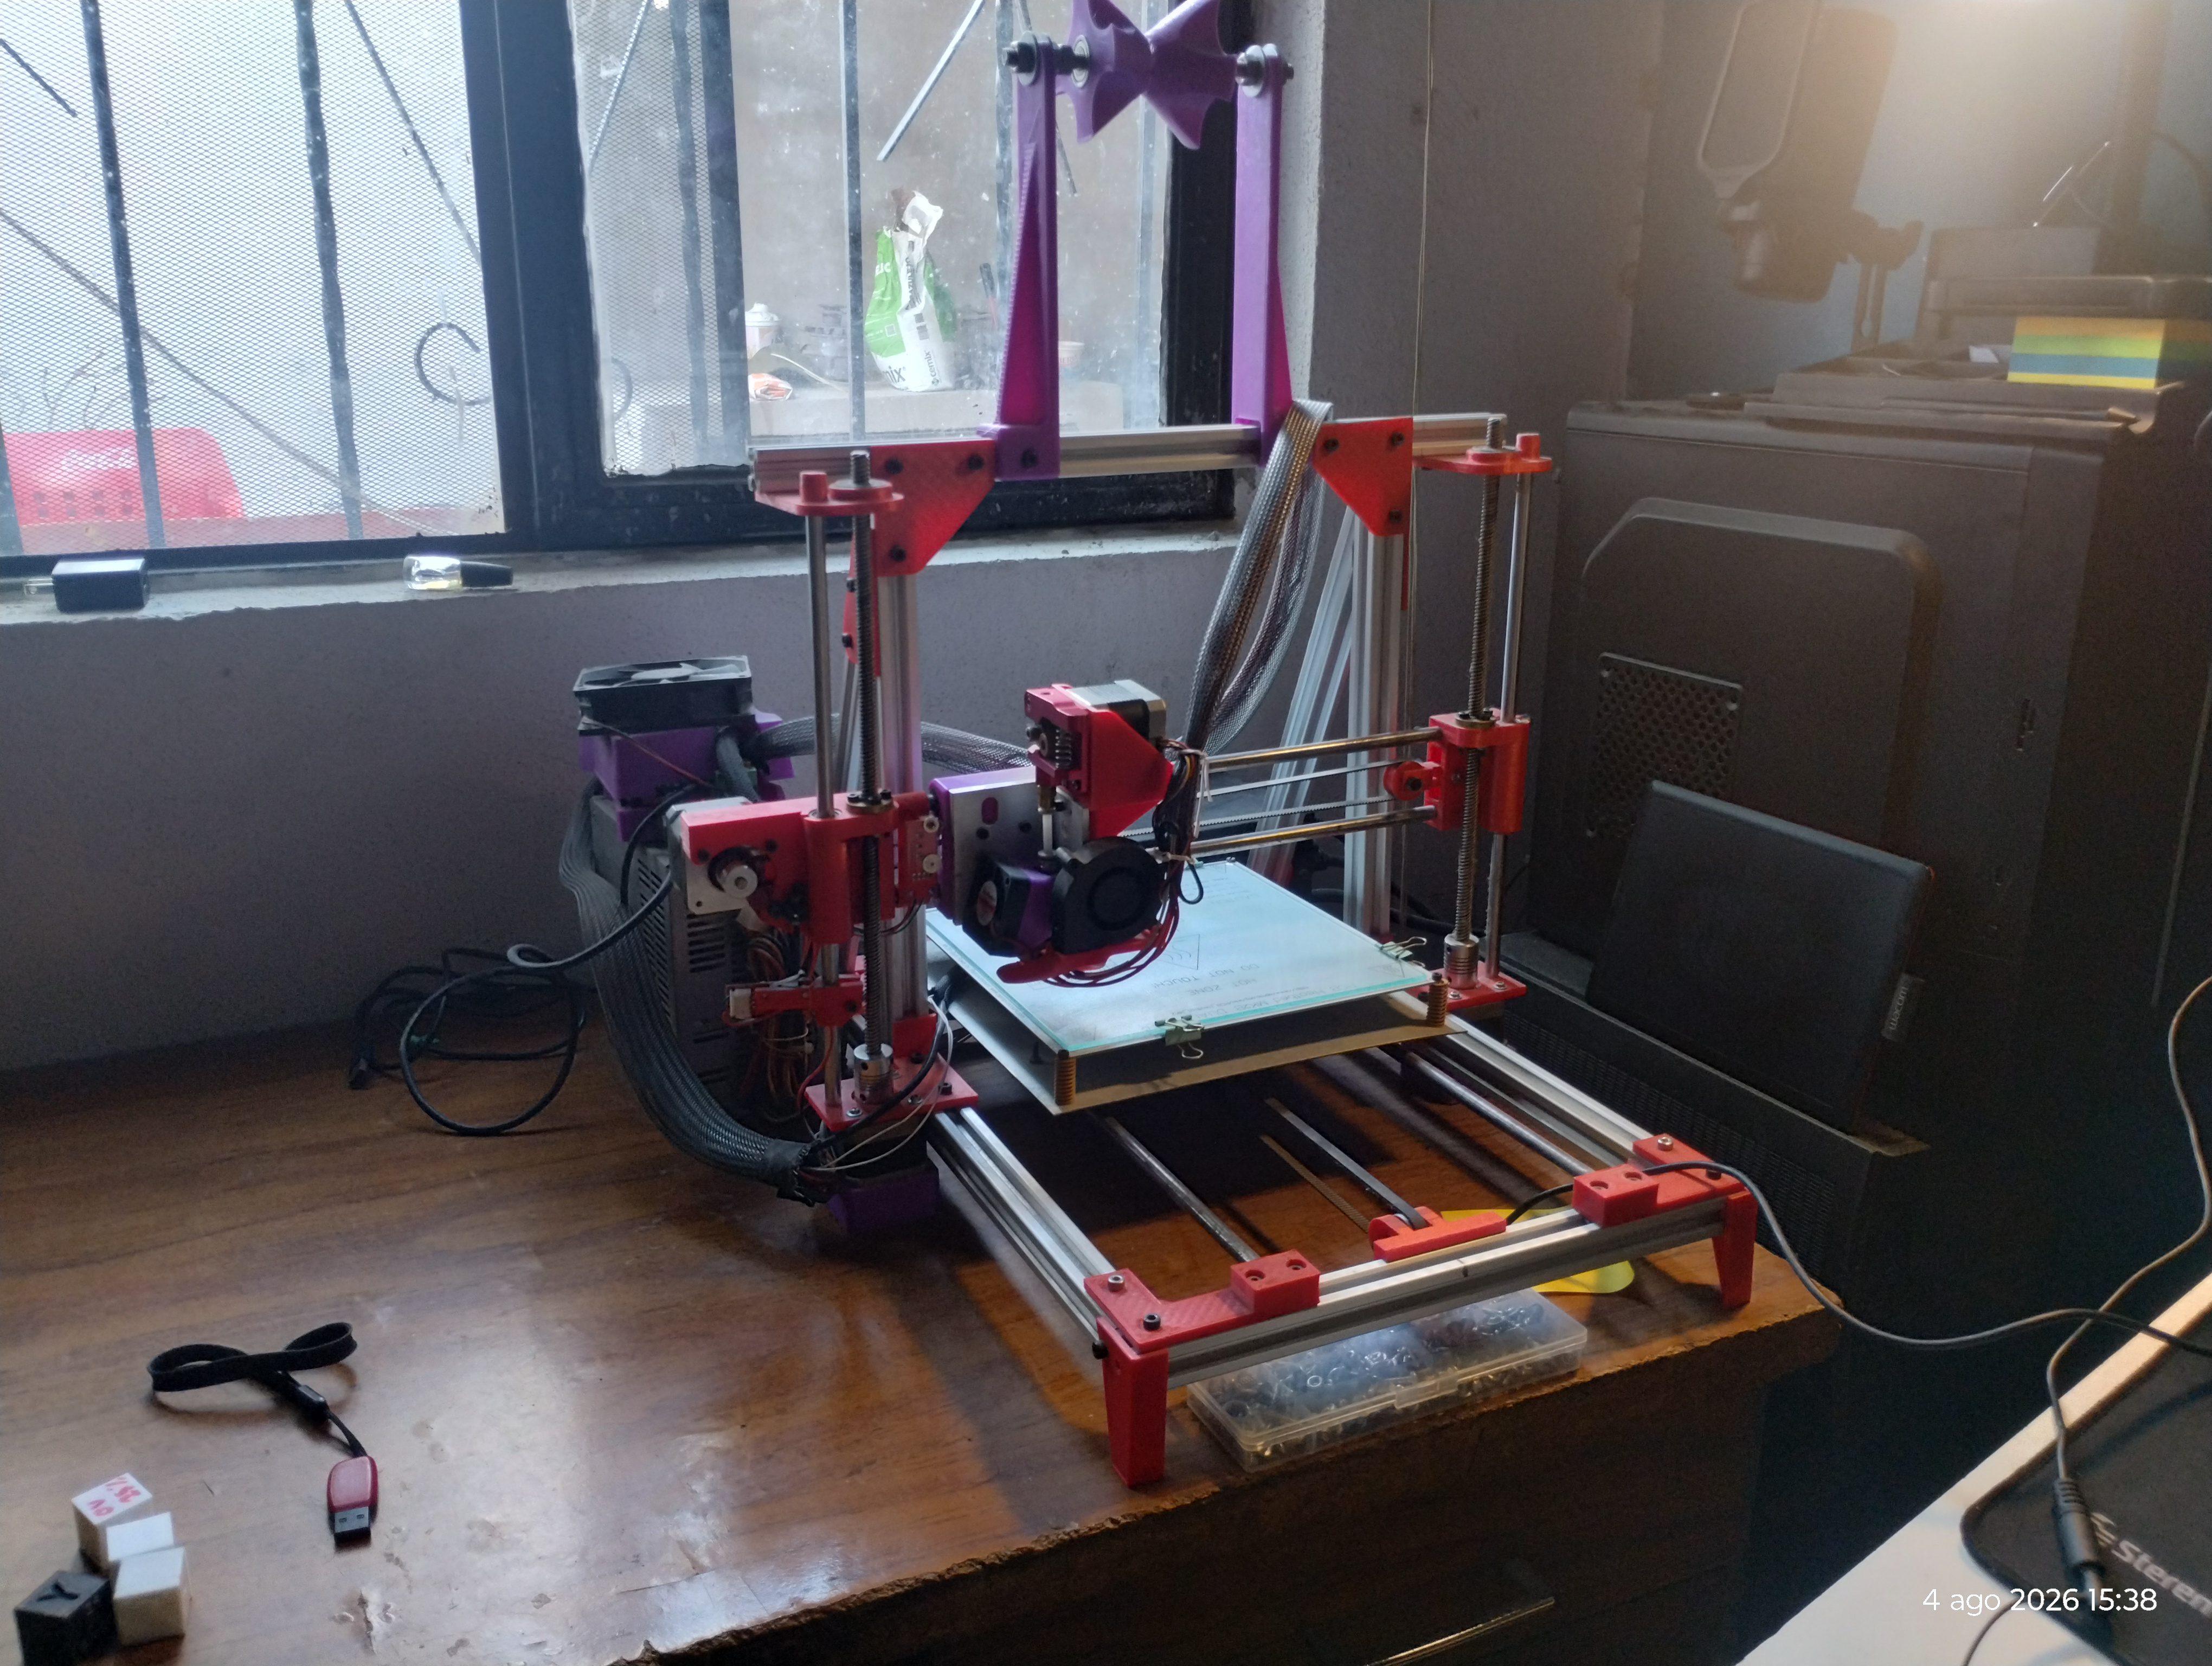
\includegraphics[width=0.5\linewidth]{Ensamblaje final.jpg}
    \caption{Ensamblaje final}
    \label{fig:ensamblaje_final}
\end{figure}

\subsection{Dimensiones y masa del equipo}
Las dimensiones generales y la masa total del equipo se presentan en la Tabla~\ref{tab:dimensiones_equipo}. Estos valores corresponden al equipo completamente ensamblado, incluyendo la estructura, la electrónica, el sistema de extrusión y la cama calefactada.

\begin{table}[htbp]
    \centering
    \caption{Dimensiones generales y masa total del equipo.}
    \label{tab:dimensiones_equipo}
    \begin{tabular}{lc}
        \toprule
        \textbf{Característica} & \textbf{Valor} \\
        \midrule
        Largo      & \qty{47}{\cm} \\
        Ancho      & \qty{52}{\cm} \\
        Alto       & \qty{57}{\cm} \\
        Masa total & \qty{7.2}{\kg} \\
        \bottomrule
    \end{tabular}
   
\end{table}

El equipo presenta dimensiones exteriores de \qty{47}{\cm} de largo, 
\qty{52}{\cm} de ancho y \qty{57}{\cm} de alto, con una masa total de 
\qty{7.2}{\kg}. Estas dimensiones permiten ubicar el equipo sobre una mesa 
de trabajo convencional y son compatibles con el espacio disponible en un 
laboratorio de prototipado.

\subsection{Componentes auxiliares integrados}

Además del módulo de extrusión, el equipo incorpora los siguientes 
componentes auxiliares:

\begin{itemize}
    \item \textbf{Escuadras de refuerzo:} instaladas en las uniones de menor 
    rigidez para reducir el juego mecánico (Figura~\ref{fig:estabilizador}).
    \item \textbf{Tensor de la correa del eje \(X\):} permite ajustar la 
    tensión de la correa después del ensamblaje 
    (Figura~\ref{fig:tensor_eje_x}).
    \item \textbf{Sistema de ajuste de finales de carrera:} permite 
    reposicionar los interruptores de límite sin desmontar la estructura 
    (Figura~\ref{fig:calibrador_altura}).
    \item \textbf{Soporte de carrete:} sostiene el carrete de filamento 
    durante la impresión.
    \item \textbf{Case del controlador:} protege la electrónica de control.
\end{itemize}


\section{Sistema de extrusión desarrollado}
\label{sec:sistema_extrusion_desarrollado}
Como resultado del proceso de diseño y fabricación, se obtuvo el módulo de extrusión mostrado en la Figura~\ref{fig:extrusor_final}, correspondiente a la configuración final integrada en la impresora. El módulo integró la base estructural de aluminio, el motor NEMA 17, el extrusor MK8, el hotend y los dos sistemas de enfriamiento del hotend y capa. La configuración corresponde a un sistema de accionamiento directo (\textit{direct drive}), en el que el motor y el mecanismo de alimentación se desplazan junto con el hotend sobre el carro del eje \(X\).
 

\begin{figure}[H]
    \centering
    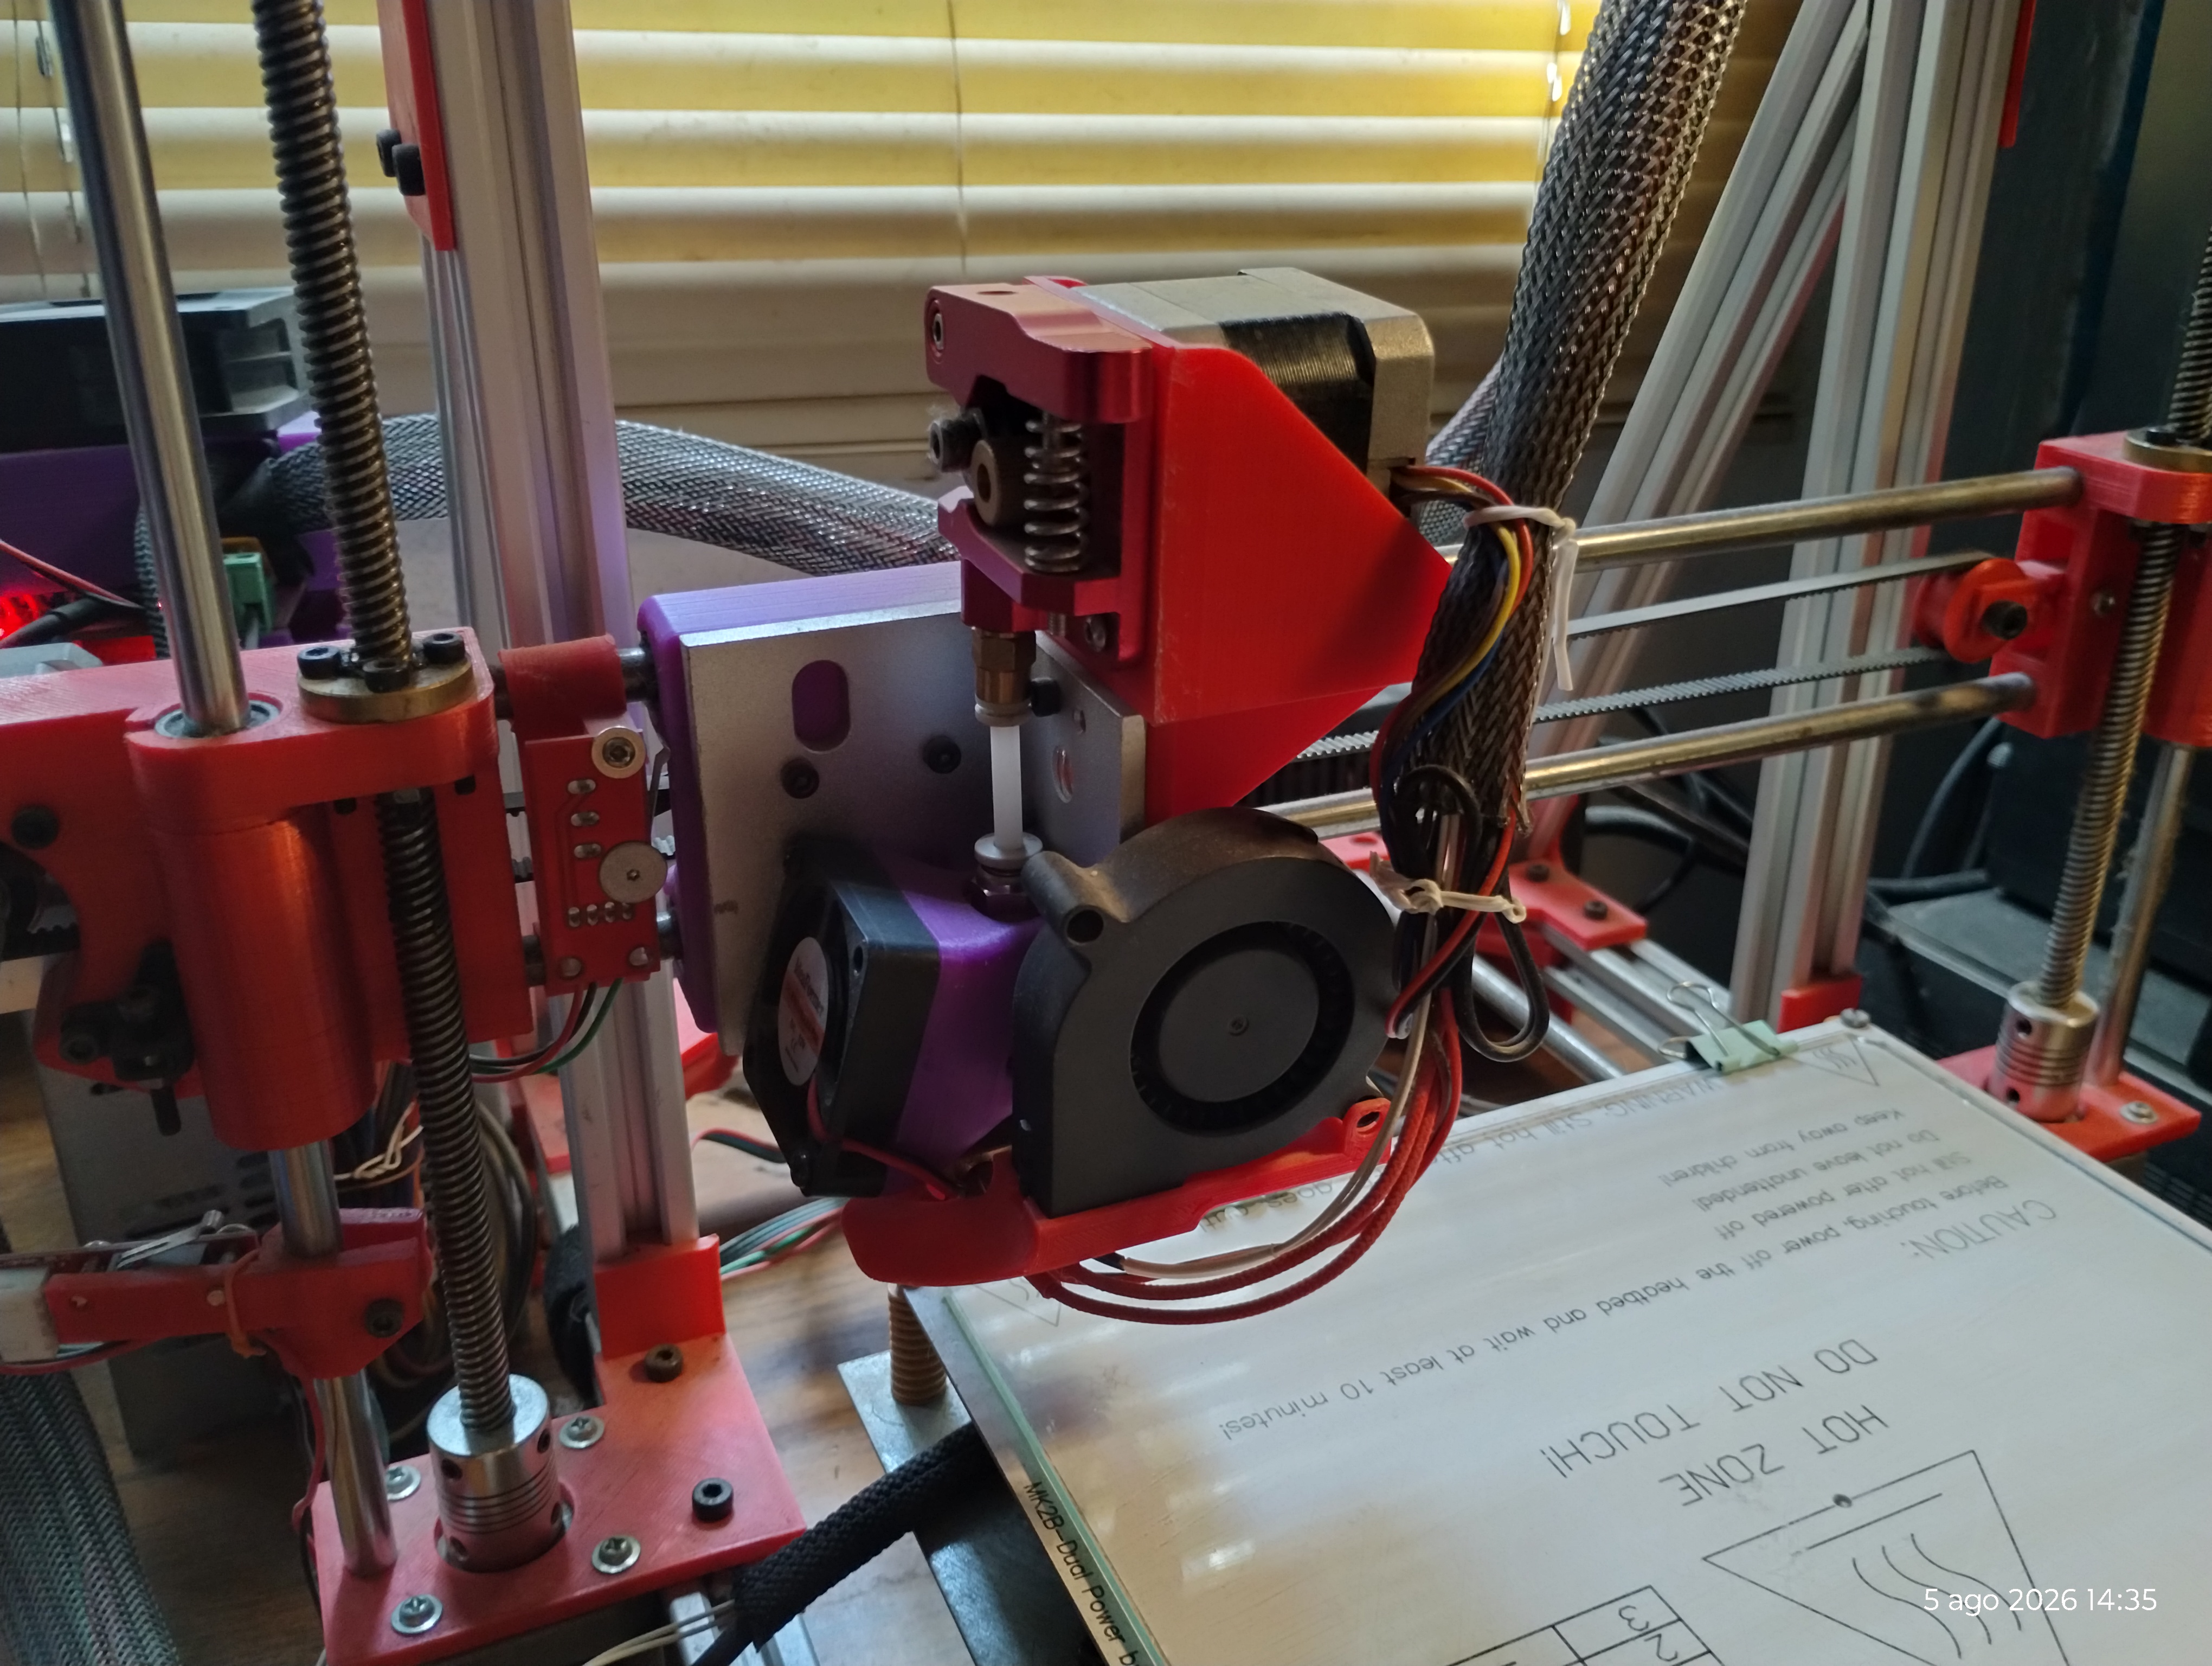
\includegraphics[width=0.5\linewidth]{Extrusor final.jpg}
    \caption{Módulo de extrusión en su configuración final.}
    \label{fig:extrusor_final}
\end{figure}


Las dimensiones generales y la masa del sistema de extrusión se presentan en la Tabla \ref{tab:comparacion_extrusion2}. Para facilitar la comparación, se incluyen los valores correspondientes a la configuración original y a la configuración rediseñada.


\begin{table}[htbp]
    \centering
    \caption{Comparación dimensional y de masa del sistema de extrusión.}
    \label{tab:comparacion_extrusion2}
    \begin{tabular}{lccc}
        \toprule
        \textbf{Característica} & \textbf{Original} & 
        \textbf{Rediseñado} & \textbf{Variación} \\
        \midrule
        Alto          & \qty{18}{\cm} & \qty{14}{\cm} & \qty{-4}{\cm} \\
        Ancho         & \qty{12}{\cm} & \qty{10}{\cm} & \qty{-2}{\cm} \\
        Largo         & \qty{9}{\cm}  & \qty{7}{\cm}  & \qty{-2}{\cm} \\
        Masa total    & \qty{650}{\g} & \qty{493}{\g} & \qty{-157}{\g} \\
        \midrule
        Recorrido Z disponible & \qty{180}{\mm} & \qty{250}{\mm} 
        & \qty{70}{\mm} \\
        \bottomrule
    \end{tabular}
\end{table}

El módulo rediseñado presentó una reducción de \qty{4}{\cm} en altura, 
\qty{2}{\cm} en ancho y \qty{2}{\cm} en largo respecto a la configuración 
original. La masa total se redujo de \qty{650}{\g} a \qty{493}{\g}, lo que 
representa una disminución de \qty{157}{\g}, equivalente al 24.2\% de la masa 
original.

\section{Validación del sistema de movimiento}
\label{sec:validacion_movimiento}

Tras aplicar el procedimiento de calibración descrito en la subsección \ref{sec:calibracion_del_sistema_de_movimiento}, se verificó la correspondencia entre el desplazamiento programado y el desplazamiento real de cada eje. Los resultados obtenidos se presentan en la Tabla \ref{tab:precision_ejes}.


\begin{table}[htbp]
    \centering
    \small
    \caption{Evaluación de la precisión dimensional y error por eje.}
    \label{tab:precision_ejes}
    \begin{tabularx}{\textwidth}{c X X X X}
        \toprule
        \textbf{Eje} & 
        \textbf{Distancia programada} & 
        \textbf{Distancia medida} & 
        \textbf{Error absoluto} & 
        \textbf{Error (\%)} \\
        \midrule
        \(X\) & \qty{100.0}{\mm} & \qty{100.2}{\mm} & \qty{0.2}{\mm} & 0.20\,\% \\
        \(Y\) & \qty{100.0}{\mm} & \qty{99.7}{\mm}  & \qty{0.3}{\mm} & 0.30\,\% \\
        \(Z\) & \qty{100.0}{\mm} & \qty{100.2}{\mm} & \qty{0.2}{\mm} & 0.20\,\% \\
        \bottomrule
    \end{tabularx}
\end{table}

Los tres ejes presentaron errores absolutos inferiores a \qty{0.5}{\mm}, 
lo que corresponde a errores relativos menores al 0.5\%. El eje \(Y\) 
presentó el error más alto (\qty{0.3}{\mm}), mientras que los ejes \(X\) y 
\(Z\) presentaron errores de \qty{0.2}{\mm} cada uno.

\subsection{Validación del sistema térmico}
\label{sec:validacion_termica}
Tras aplicar el procedimiento de calibración descrito en la 
sección~\ref{sec:calibracion_termica}, se obtuvieron las constantes de 
control PID para el hotend y para la cama calefactada. La 
Tabla~\ref{tab:pid_final} presenta los valores finales incorporados al 
firmware.

% ============================================================
% CÓMO OBTENER LAS CONSTANTES PID:
% 
% Opción A (desde la impresora):
%   1. Conectar la impresora a Pronterface, OctoPrint o similar.
%   2. Enviar el comando M503 (reporta la configuración actual).
%   3. Buscar las líneas:
%      M301 P... I... D...   (para el hotend)
%      M304 P... I... D...   (para la cama calefactada)
%   4. Anotar los valores de P, I, D.
%
% Opción B (ejecutar autotune de nuevo):
%   1. Enviar M303 E0 S200 C8   (hotend a 200°C, 8 ciclos)
%   2. Enviar M303 E-1 S60 C8   (cama a 60°C, 8 ciclos)
%   3. Marlin reporta los valores al final de cada autotune.
%   4. Anotar los valores y guardarlos con M500.
% ============================================================


\begin{table}[htbp]
    \centering
    \caption{Constantes PID obtenidas para el hotend y la cama calefactada.}
    \label{tab:pid_final}
    \begin{tabular}{lccc}
        \toprule
        \textbf{Componente} & \textbf{$K_p$} & 
        \textbf{$K_i$} & \textbf{$K_d$} \\
        \midrule
        Hotend        & [dato] & [dato] & [dato] \\
        Cama calefactada & [dato] & [dato] & [dato] \\
        \bottomrule
    \end{tabular}
\end{table}

% ============================================================
% CÓMO OBTENER LAS TABLAS DE TEMPERATURA PROGRAMADA VS ALCANZADA:
%
% Estas pruebas verifican la precisión del control en estado estable.
% 
% Procedimiento para el hotend:
%   1. Enviar M104 S200  (o usar el menú de la impresora para fijar 200°C)
%   2. Esperar 2 minutos a que se estabilice.
%   3. Leer la temperatura actual desde la pantalla o con M105.
%   4. Anotar el valor.
%   5. Repetir con 210°C y 220°C.
%
% Procedimiento para la cama:
%   Igual, pero con M140 S60, luego S70 y S80.
%   La cama tarda más en estabilizarse, esperar 5 minutos.
%
% Toma al menos 3 lecturas por temperatura y promedia.
% ============================================================

La Tabla~\ref{tab:temp_hotend} presenta las temperaturas programadas y 
alcanzadas en el hotend para tres valores de referencia, mientras que la 
Tabla~\ref{tab:temp_cama} presenta los resultados equivalentes para la cama 
calefactada.

\begin{table}[htbp]
    \centering
    \caption{Temperatura programada frente a alcanzada en el hotend.}
    \label{tab:temp_hotend}
    \begin{tabular}{ccc}
        \toprule
        \textbf{Prueba / Ensayo} & \textbf{Temp. Programada} & \textbf{Temp. Alcanzada} \\
        \midrule
        1 & \qty{200}{\celsius} & \qty{200.2}{\celsius} \\
        2 & \qty{210}{\celsius} & \qty{210.1}{\celsius} \\
        3 & \qty{220}{\celsius} & \qty{220.0}{\celsius} \\
        \bottomrule
    \end{tabular}
\end{table}

\begin{table}[htbp]
    \centering
    \caption{Temperatura programada frente a alcanzada en la cama caliente.}
    \label{tab:temp_cama}
    \begin{tabular}{ccc}
        \toprule
        \textbf{Prueba / Ensayo} & \textbf{Temp. Programada} & \textbf{Temp. Alcanzada} \\
        \midrule
        1 & \qty{60}{\celsius} & \qty{59.8}{\celsius} \\
        2 & \qty{70}{\celsius} & \qty{70.1}{\celsius} \\
        3 & \qty{80}{\celsius} & \qty{80.2}{\celsius} \\
        \bottomrule
    \end{tabular}
\end{table}

% ============================================================
% CÓMO OBTENER LA GRÁFICA DE TEMPERATURA VS TIEMPO:
%
% Esta prueba mide la estabilidad dinámica durante la impresión real.
%
% Método 1 (con Pronterface / OctoPrint):
%   1. Cargar una pieza de prueba (ej. cubo de 20x20x20 mm).
%   2. En Pronterface: pestaña "Temperature Graph" o 
%      en OctoPrint: pestaña "Temperature".
%   3. Iniciar la impresión.
%   4. La gráfica se genera automáticamente.
%   5. Capturar la pantalla después de 10-15 min de impresión.
%
% Método 2 (registro manual):
%   1. Durante la impresión, enviar M105 cada 30 segundos.
%   2. Anotar: tiempo, temperatura actual, temperatura objetivo.
%   3. Repetir durante 10-15 minutos.
%   4. Graficar en Excel o Python (tiempo vs temperatura).
%
% Análisis a reportar:
%   - Variación máxima (temp. máx - temp. mín).
%   - Desviación estándar.
%   - Si la variación es ≤ ±2°C, el control es estable.
% ============================================================

La Figura~\ref{fig:grafica_temperatura} presenta el comportamiento de la temperatura del hotend durante una impresión de prueba de 15 minutos. El registro se realizó con el software [COMPLETAR: Pronterface/OctoPrint/Otro].

\begin{comment}
\begin{figure}[H]
    \centering
    \includegraphics[width=0.8\linewidth]{Grafica_temperatura_hotend.png}
    \caption{Respuesta térmica del hotend durante la impresión.}
    \label{fig:grafica_temperatura}
\end{figure}
\end{comment}


Durante el período registrado, la temperatura del hotend se mantuvo dentro de un rango de \qty{\pm 0000}{\celsius} respecto a la temperatura de referencia, con una desviación estándar de \qty{0000}{\celsius}. Este resultado indica que el lazo de control mantiene la temperatura estable incluso ante las demandas dinámicas del proceso de extrusión.

% ============================================================
% CÓMO OBTENER EL TIEMPO DE CALENTAMIENTO:
%
% Procedimiento:
%   1. Con la impresora a temperatura ambiente (registrar la temp. inicial).
%   2. Enviar M104 S200 y arrancar un cronómetro.
%   3. Detener el cronómetro cuando la temperatura alcance 200°C.
%   4. Anotar el tiempo.
%   5. Repetir con la cama: M140 S60, medir tiempo hasta 60°C.
% ============================================================

La Tabla~\ref{tab:tiempo_calentamiento} presenta el tiempo requerido por 
cada componente para alcanzar su temperatura de operación desde temperatura 
ambiente, así como la variación en estado estable una vez alcanzada la 
referencia.

\begin{comment}
    

\begin{table}[htbp]
    \centering
    \caption{Tiempo de calentamiento y variación en estado estable.}
    \label{tab:tiempo_calentamiento}
    \begin{tabular}{lcc}
        \toprule
        \textbf{Componente} & \textbf{Tiempo de calentamiento} & 
        \textbf{Variación en estado estable} \\
        \midrule
        Hotend        & [dato] s & \(\pm\)[dato]\celsius \\
        Cama calefactada & [dato] s & \(\pm\)[dato]\celsius \\
        \bottomrule
    \end{tabular}
\end{table}


\begin{comment}
    

     \begin{table}[htbp]
    \centering
    \caption{Tabla de tiempo de calentamiento y variación en estado estable para hotend y cama.}
    \label{tab:temp_cama3}
    \begin{tabular}{ccc}
        \toprule
        \textbf{Prueba / Ensayo} & \textbf{Temp. Programada} & \textbf{Temp. Alcanzada} \\
        \midrule
        1 & \qty{60}{\celsius} & \qty{59.8}{\celsius} \\
        2 & \qty{70}{\celsius} & \qty{70.1}{\celsius} \\
        3 & \qty{80}{\celsius} & \qty{80.2}{\celsius} \\
        \bottomrule
    \end{tabular}
\end{table}

\end{comment}   


\section{Validación del sistema de extrusión}
\label{sec:validacion_extrusion}

Tras aplicar el procedimiento de calibración descrito en la 
sección~\ref{sec:calibracion_extrusor}, se verificó la cantidad de filamento 
suministrada por el mecanismo de alimentación. La 
Tabla~\ref{tab:calibracion_extrusor} presenta los resultados de la prueba de 
verificación.

% ============================================================
% CÓMO OBTENER LOS DATOS:
%
% Esta prueba ya la hiciste durante la calibración (sección 6.6.3).
% Solo necesitas recuperar los valores que anotaste:
%   - Longitud programada: 100 mm
%   - Longitud medida: [el valor real que mediste]
%   - Error absoluto: [programada - medida]
%   - Error (%): [(error absoluto / programada) × 100]
%   - Pasos/mm finales: [el valor que quedó en el firmware]
% ============================================================

\begin{table}[htbp]
    \centering
    \caption{Verificación de la calibración del extrusor.}
    \label{tab:calibracion_extrusor}
    \begin{tabular}{lcc}
        \toprule
        \textbf{Parámetro} & \textbf{Valor} \\
        \midrule
        Longitud programada          & \qty{100}{\mm} \\
        Longitud medida              & [dato] \unit{\mm} \\
        Error absoluto               & [dato] \unit{\mm} \\
        Error relativo               & [dato]\,\% \\
        Pasos por milímetro finales  & [dato] \\
        \bottomrule
    \end{tabular}
\end{table}

% ============================================================
% CÓMO VERIFICAR LA AUSENCIA DE DEFORMACIÓN DEL SOPORTE:
%
% Procedimiento:
%   1. Imprimir una pieza de prueba de al menos 30 minutos de duración.
%   2. Al terminar, revisar visualmente el soporte del motor y la base 
%      de aluminio.
%   3. Verificar que no haya deformación, decoloración ni 
%      desprendimiento.
%   4. Opcional: medir la temperatura del soporte con termopar 
%      después de 30 min de impresión.
%
% Si el soporte no presentó deformación, indícalo. Si presentó 
% alguna, descríbela.
% ============================================================

Adicionalmente, se monitoreó el estado del soporte del motor y de la base 
estructural durante la fabricación de las piezas del proyecto (algunas de las 
cuales requirieron varias horas de impresión). A diferencia de la primera 
iteración, en la que el soporte de PLA se deformó por la transferencia de 
calor, en esta configuración final no se observó deformación, decoloración ni 
pérdida de rigidez en los componentes poliméricos. Esto confirma que la 
separación térmica proporcionada por la base de aluminio y la ventilación 
forzada cumplen su función durante la operación normal del equipo.

\section{Validación del sistema de enfriamiento}
\label{sec:validacion_enfriamiento}

El sistema de enfriamiento del hotend tiene como propósito evacuar el calor residual del disipador para evitar que se propague hacia la zona fría del hotend y provoque el ablandamiento prematuro del filamento (\textit{heat creep}). Para evaluar la efectividad del sistema desarrollado, se realizaron mediciones de temperatura en el disipador del hotend bajo distintas condiciones de disipación.

Para las mediciones se utilizó un termopar tipo K colocado en la superficie 
externa del disipador del hotend, a media altura. La Figura~\ref{fig:posicion_sensor} muestra la ubicación exacta del sensor. En todas las pruebas se mantuvo el mismo punto de medición y se esperó un tiempo de 5 minutos a que la temperatura se estabilizara antes de registrar cada lectura. La temperatura del bloque calefactor se mantuvo en \qty{200}{\celsius} como referencia en todos los casos.

La Tabla~\ref{tab:disipacion} presenta las temperaturas registradas en el disipador bajo cada condición evaluada.

\begin{table}[htbp]
    \centering
    \caption{Temperaturas registradas en el disipador del hotend bajo distintas condiciones de disipación.}
    \label{tab:disipacion}
    \begin{tabular}{lcc}
        \toprule
        \textbf{Condición} & \textbf{Temperatura en disipador} & 
        \textbf{Temperatura en bloque calefactor} \\
        \midrule
        Sin disipador ni ventilador & \qty{71}{\celsius} & \qty{200}{\celsius} \\
        Con base de aluminio, sin ventilador & \qty{41}{\celsius} & \qty{200}{\celsius} \\
        Con base de aluminio y ventilador & \qty{47}{\celsius} & \qty{200}{\celsius} \\
        \bottomrule
    \end{tabular}
\end{table}

La incorporación de la base estructural de aluminio redujo la temperatura 
del disipador de \qty{71}{\celsius} a \qty{41}{\celsius}, lo que representa 
una disminución de \qty{30}{\celsius}, equivalente a una reducción del 
42.25\% respecto a la condición sin disipación. La adición del ventilador 
redujo la temperatura en \qty{11111}{\celsius} adicionales, alcanzando un valor final de \qty{11111}{\celsius} y una reducción total del 99\% respecto a la condición inicial.


\begin{figure}[H]
    \centering
    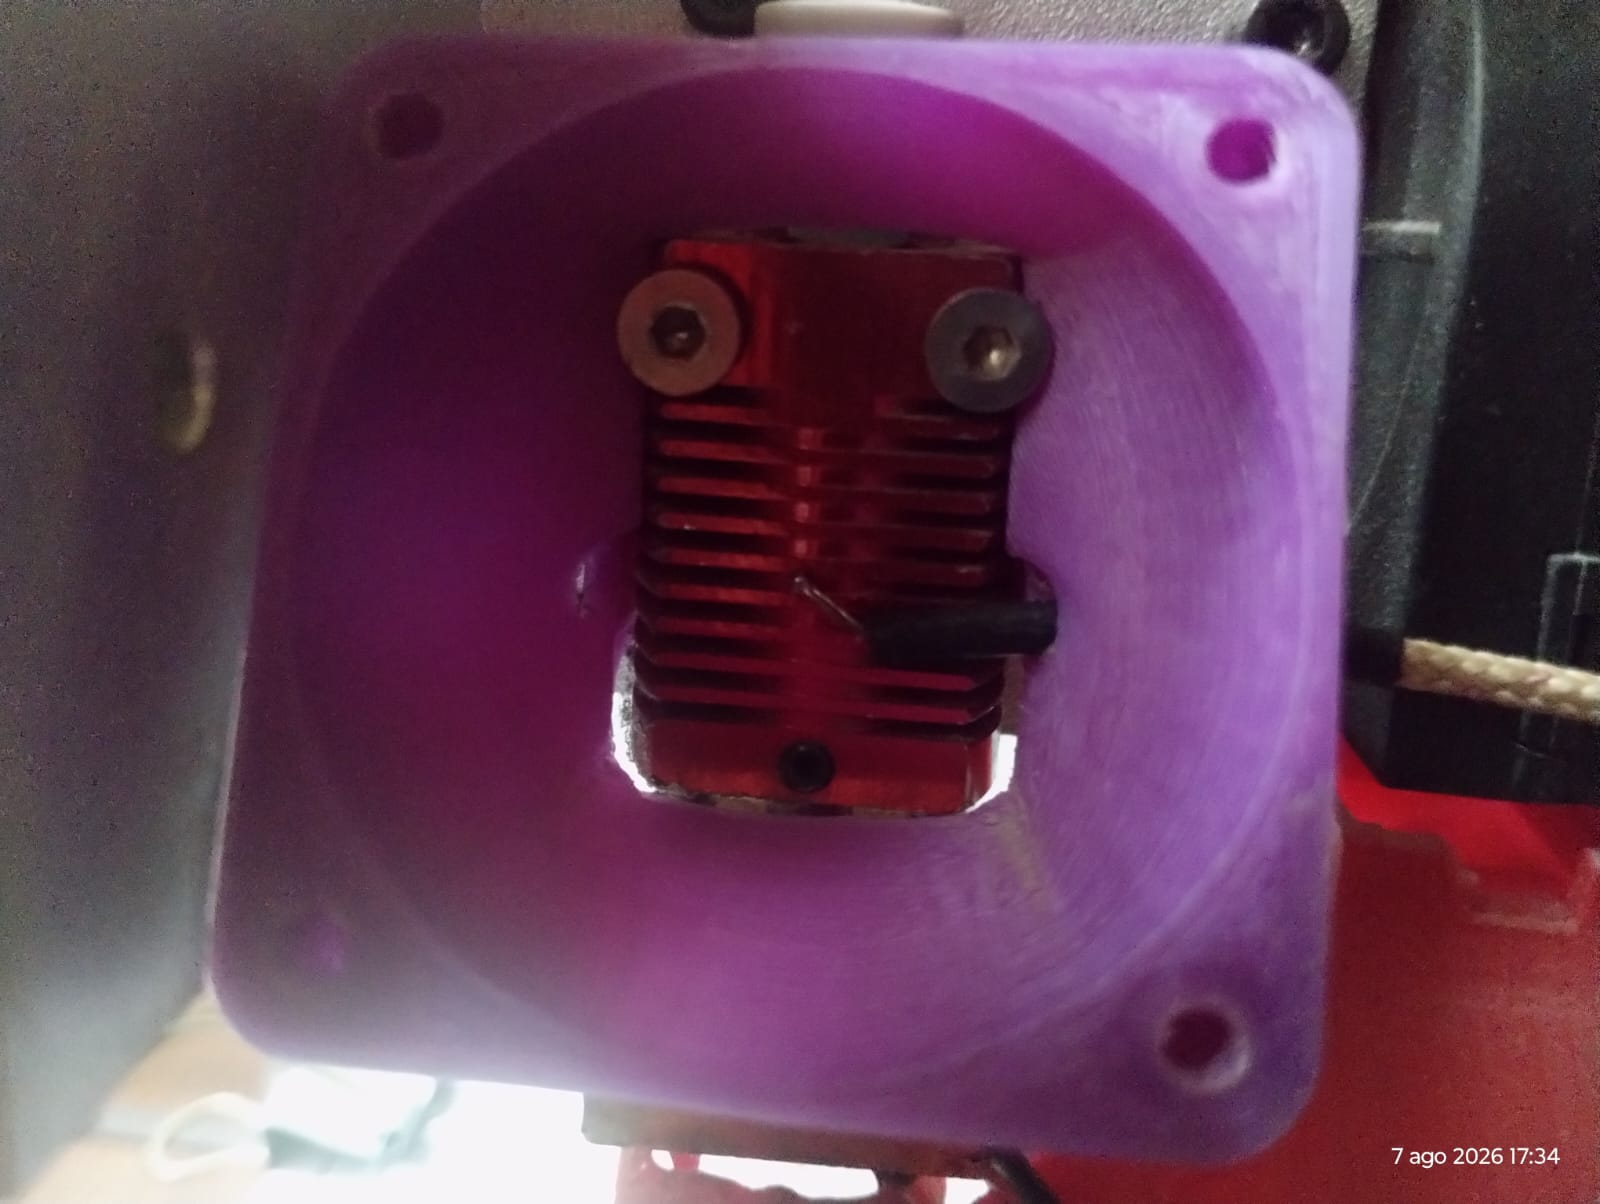
\includegraphics[width=0.5\linewidth]{Evidencia_posicion_sensor.jpeg}
    \caption{Evidencia posicionamiento de sensor de pruebas}
    \label{fig:posicion_sensor}
\end{figure}

\section{Evaluación de calidad de impresión}

\subsection{Precisión dimensional}

Evaluando la precisión del equipo conseguido se llegaron a los valores mostrados en la Tabla~\ref{tab:cubos_calibracion}. Donde estan enlistadas las dimensiones de cubos de prueba. Las dimensiones se midieron con un vernier marca Truper con resolución de \qty{0.02}{\mm}. 

\begin{table}[htbp]
    \centering
    \caption{Dimensiones y errores de los cubos de calibración.}
    \label{tab:cubos_calibracion}
    \begin{tabular}{lcccc}
        \toprule
        \textbf{Eje} & \textbf{Dimensión CAD} & \textbf{Dimensión medida} & \textbf{Error (mm)} & \textbf{Error (\%)} \\
        \midrule
        \(X\) & \qty{20.00}{\mm} & \qty{20.30}{\mm} & \qty{+0.30}{\mm} & +1.50\% \\
        \(Y\) & \qty{20.00}{\mm} & \qty{20.10}{\mm} & \qty{+0.10}{\mm} & +0.50\% \\
        \(Z\) & \qty{20.00}{\mm} & \qty{20.14}{\mm} & \qty{+0.14}{\mm} & +0.70\% \\
        \bottomrule
    \end{tabular}
\end{table}


\subsection{Pruebas geométricas}
\label{subsec:pruebas_geometricas}

Se realizaron pruebas geométricas estándar para evaluar la capacidad del 
sistema de imprimir geometrías complejas. Las pruebas incluyeron overhang, 
stringing y una torre de temperatura. Las Figuras~\ref{fig:overhang} a \ref{fig:torre_temperatura} muestran las piezas obtenidas.

\begin{figure}[H]
    \centering
    \begin{subfigure}[b]{0.45\linewidth}
        \centering
        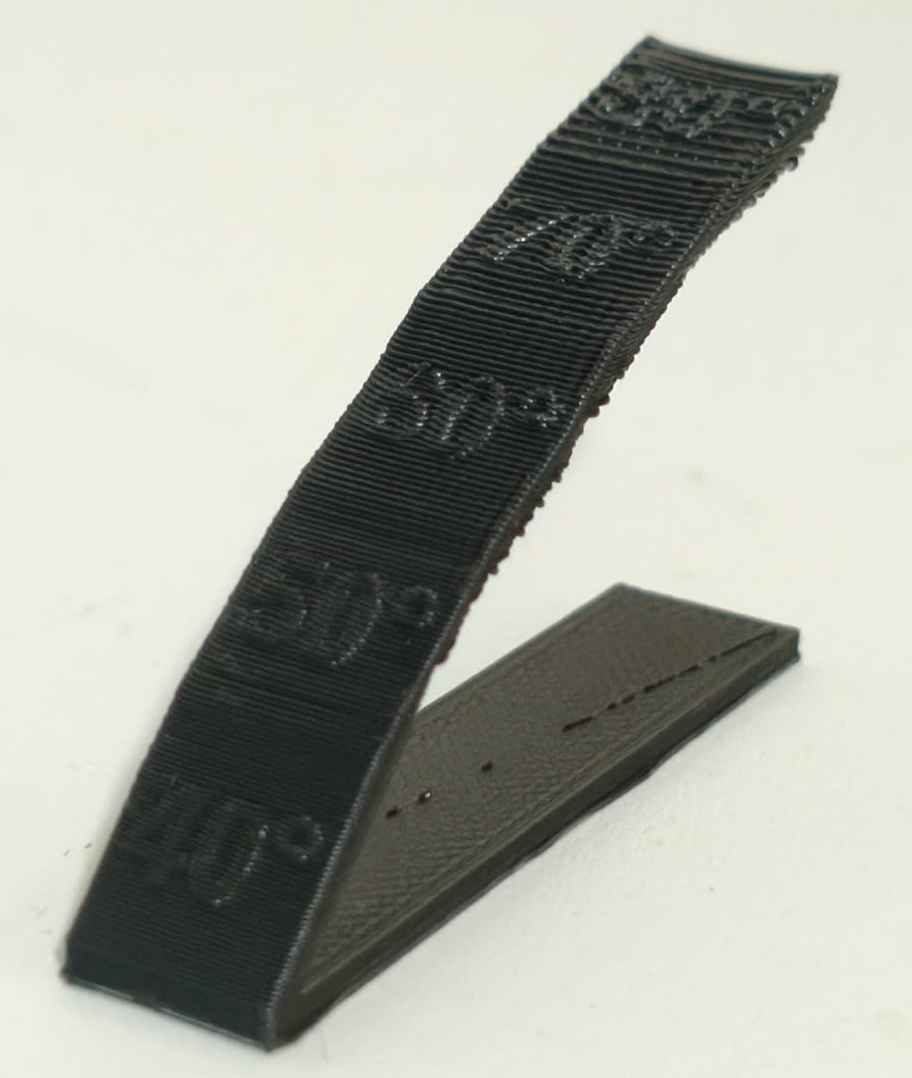
\includegraphics[width=\linewidth]{overhang.jpg}
        \caption{Prueba de overhang.}
        \label{fig:overhang}
    \end{subfigure}
    \hfill
    \begin{subfigure}[b]{0.4\linewidth}
        \centering
        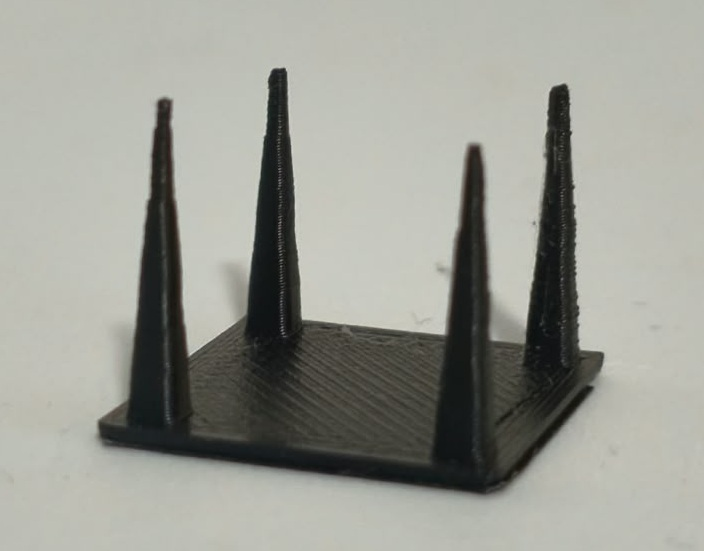
\includegraphics[width=\linewidth]{stringing.jpg}
        \caption{Prueba de stringing.}
        \label{fig:stringing}
    \end{subfigure}
    \caption{Pruebas geométricas: overhang (izquierda) y stringing (derecha).}
    \label{fig:pruebas_overhang_stringing}
\end{figure}

\begin{figure}[H]
    \centering
    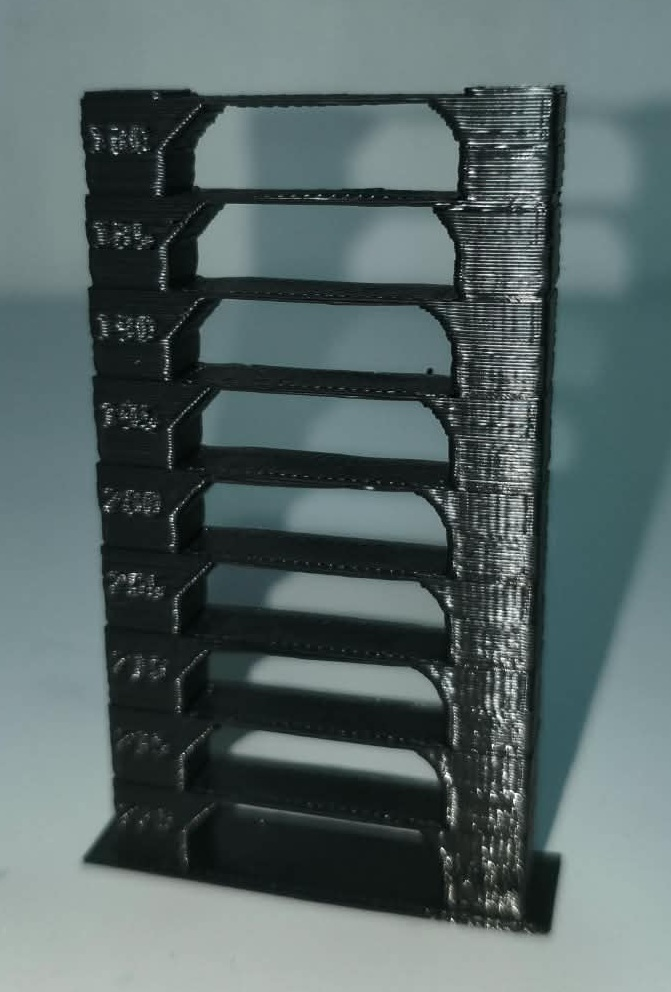
\includegraphics[width=0.5\linewidth]{torre_temperatura.jpg}
    \caption{Torre de temperatura.}
    \label{fig:torre_temperatura}
\end{figure}

\textbf{Overhang:} La pieza de prueba consistió en una geometría escalonada que varió desde \ang{40} hasta \ang{80} en incrementos de \ang{10}. Hasta \ang{70} la pieza no presentó deflexión apreciable. A partir de ese ángulo se observó un incremento en la visibilidad de las líneas de capa, que se 
acentuó a \ang{80}. No obstante, en ningún caso se produjo el colapso de la estructura, por lo que el sistema mantuvo la continuidad de la impresión en toda la pieza.

\textbf{Stringing:} La pieza de prueba consistió en cuatro torres separadas. No se observó formación significativa de hilos entre las torres; únicamente se apreciaron un par de filamentos muy finos que no resultaron visibles en la fotografía. Las torres conservaron su forma y sus dimensiones sin presentar defectos apreciables.

\textbf{Torre de temperatura:} La torre se imprimió en un rango de \qty{220}{\celsius} en la base hasta \qty{180}{\celsius} en la parte superior, con decrementos de \qty{5}{\celsius} por escalón. A simple vista, todos los escalones presentaron una impresión satisfactoria. Sin embargo, al inspeccionar la pieza a contraluz se observaron diferencias notables entre los escalones.

Los escalones correspondientes al rango de \qty{210}{\celsius} a 
\qty{220}{\celsius} presentaron translucidez, lo que permitió observar a través de la pieza. Los escalones inferiores, correspondientes al rango de \qty{180}{\celsius} a \qty{190}{\celsius}, mostraron ligeros defectos superficiales. El escalón correspondiente a \qty{205}{\celsius} presentó la mejor combinación de acabado superficial y uniformidad, por lo que este valor se adoptó como temperatura de referencia para las impresiones posteriores.

\subsection{Problemas de impresión presentados y soluciones}
\label{subsec:problemas_soluciones}

A lo largo del desarrollo de las pruebas de impresión se presentaron diversas 
problemáticas que requirieron ajustes iterativos. Dado que las pruebas se 
realizaron en distintas etapas del proyecto y con diferentes materiales, los 
problemas y sus soluciones se describen a continuación de forma cronológica.

\textbf{Ajuste inicial y evolución de la calidad:} Durante las primeras 
fases de calibración, se imprimieron múltiples cubos de prueba para afinar 
los parámetros del laminador. En la Figura~\ref{fig:evolucion_cubos} se 
observa una comparación entre dos cubos impresos consecutivamente con 
configuraciones distintas, donde se aprecia una mejora sustancial en la 
uniformidad de las paredes, la definición de las esquinas y la precisión 
dimensional.

\begin{figure}[h]
    \centering
    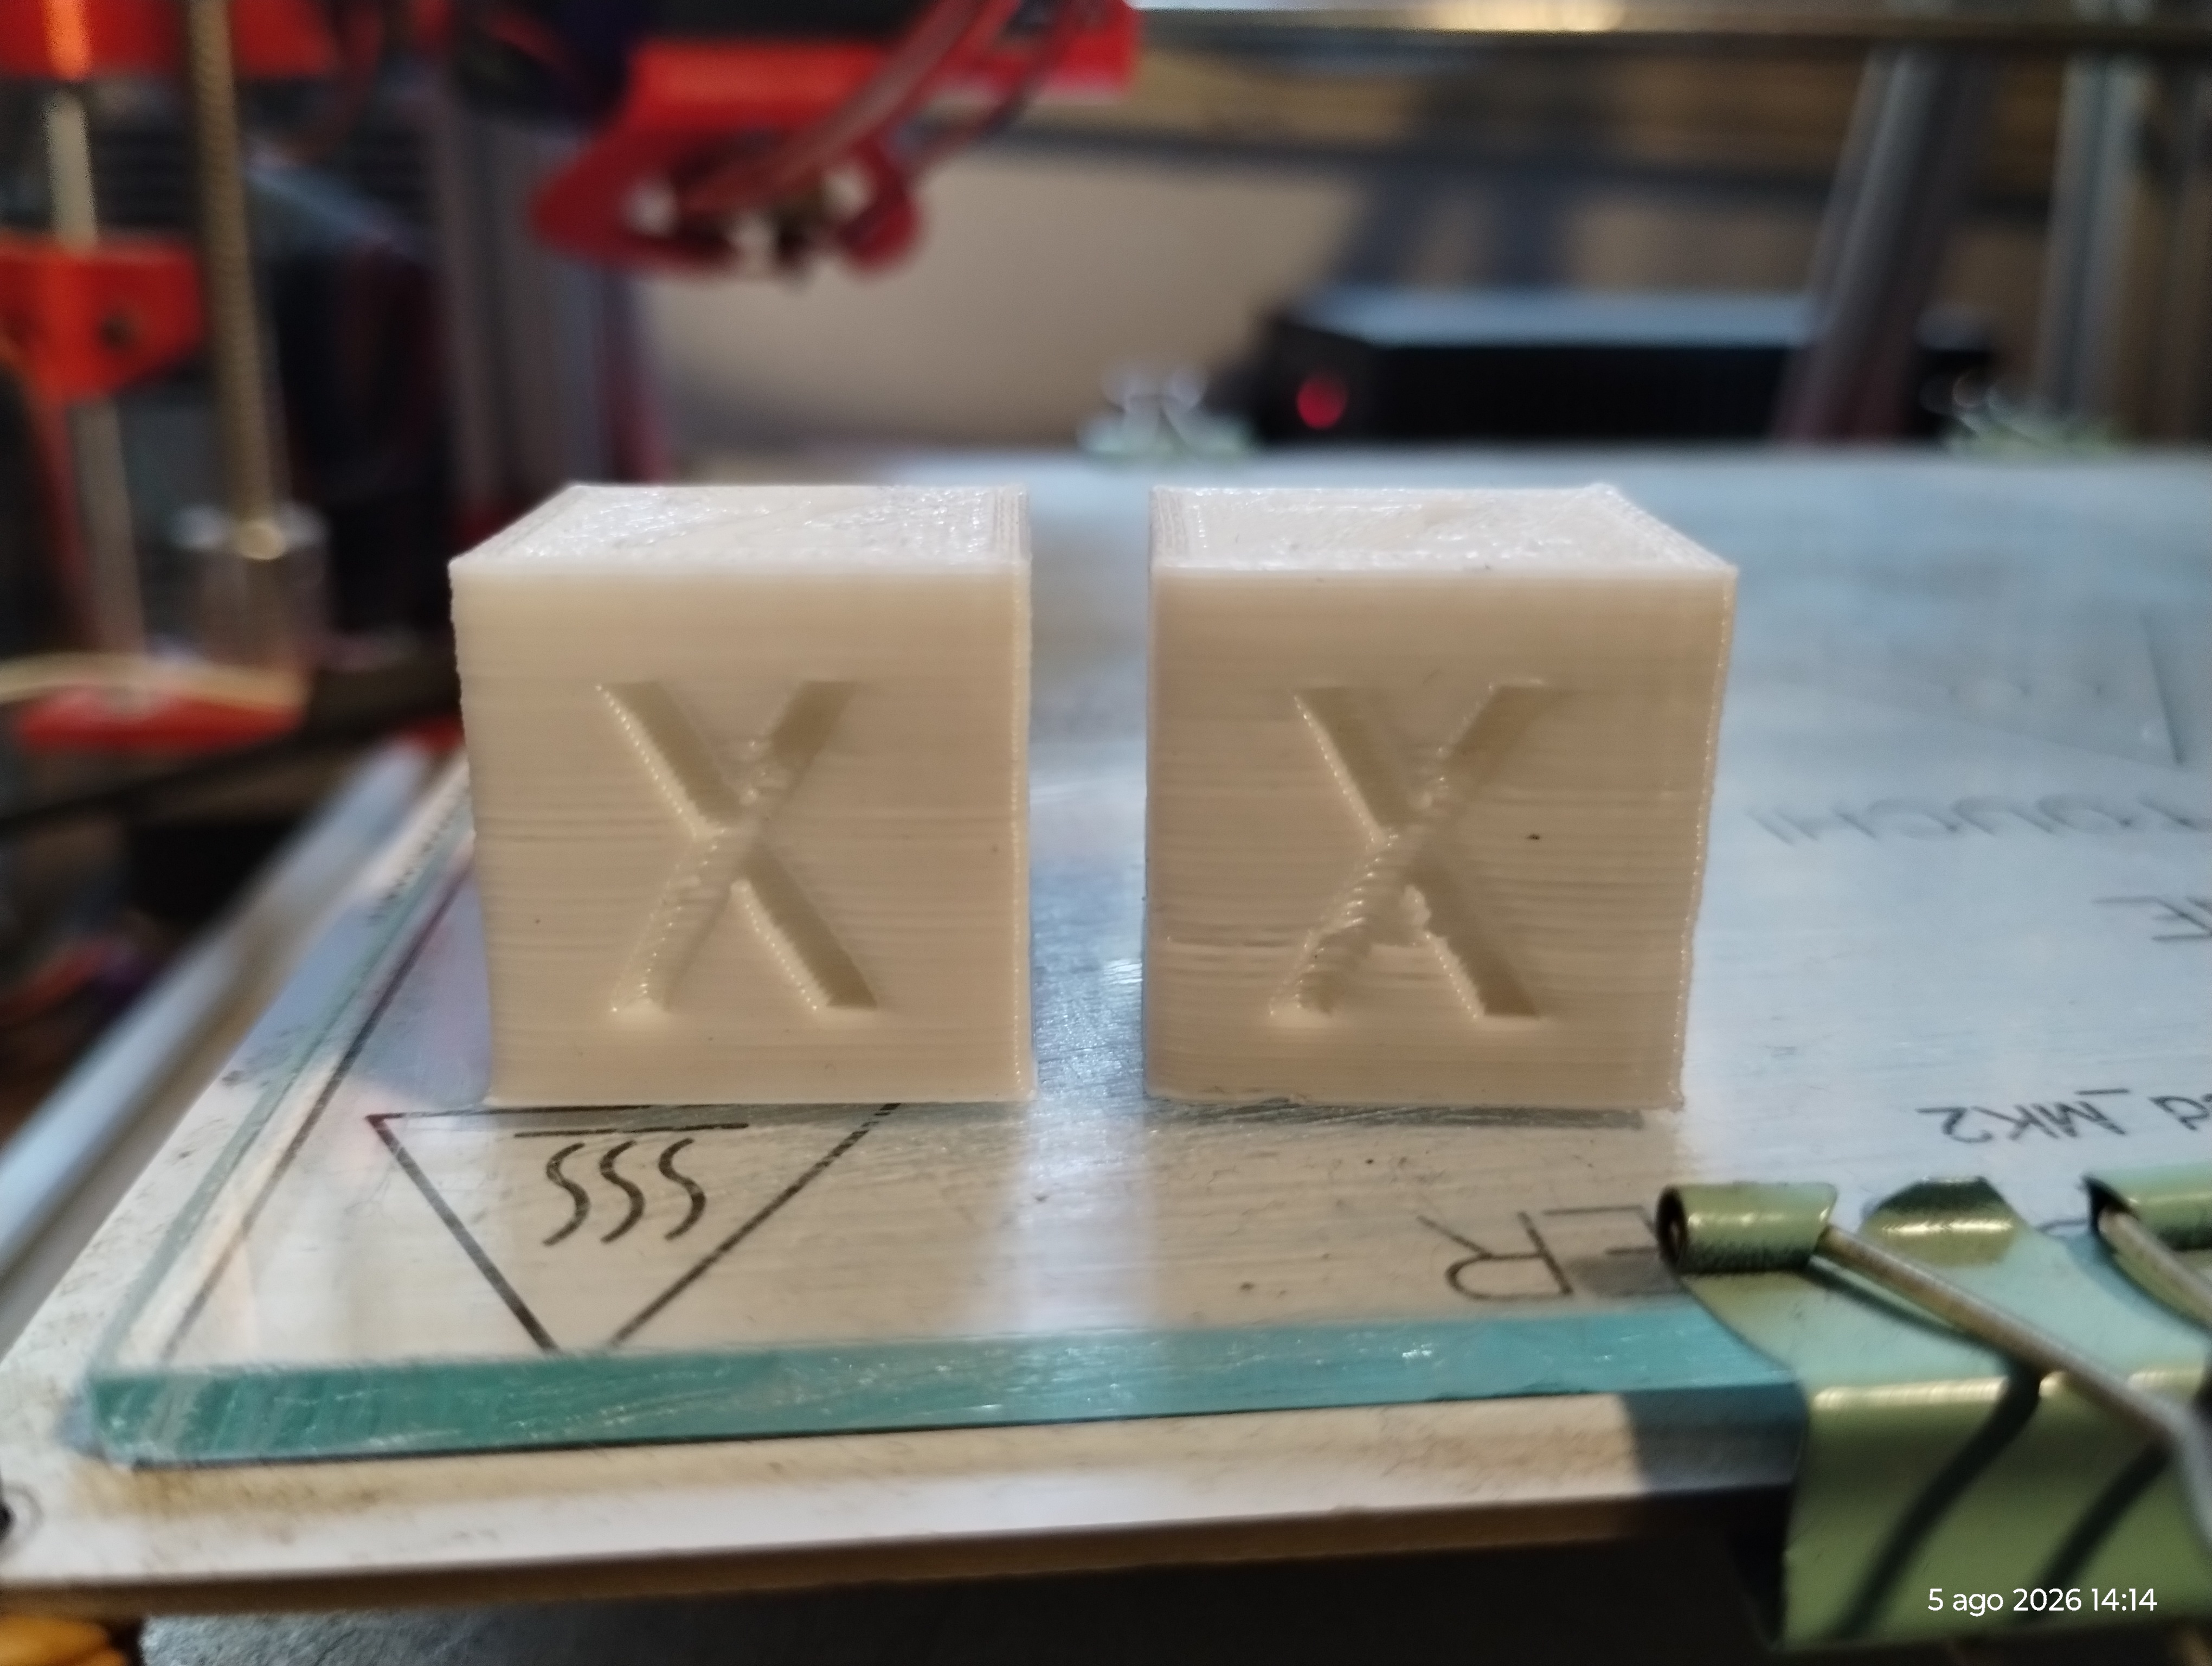
\includegraphics[width=0.5\linewidth]{comparacion calidad.jpg}
    \caption{Comparación entre dos cubos de calibración impresos con diferentes parámetros de configuración.}
    \label{fig:evolucion_cubos}
\end{figure}

\textbf{Diagnóstico de humedad en el filamento:} Tras un periodo de 
impresiones exitosas, la calidad de las piezas comenzó a deteriorarse 
repentinamente. Se verificó que los parámetros del software no se habían 
modificado y que la impresora no presentaba fallas mecánicas (como 
atascamientos o pérdida de pasos). Los síntomas observados en las piezas 
fueron una mayor fragilidad y un acabado superficial inusualmente brillante. 
Tras consultar literatura técnica y foros especializados, se identificó que 
estos síntomas eran característicos de la humedad absorbida por el filamento 
de PLA.

Para comprobar esta hipótesis, se realizó una prueba de control sustituyendo 
el carrete por un filamento nuevo de otra marca. Las impresiones mejoraron 
significativamente desde la primera prueba, lo que confirmó que el problema 
no era mecánico ni de configuración, sino que el filamento anterior había 
absorbido humedad del ambiente. No obstante, el nuevo material requirió un 
ajuste fino en los parámetros del laminador para alcanzar la calidad óptima, 
lo que evidenció que cada marca de filamento posee características propias.

\textbf{Solución aplicada:} Al desconocer inicialmente las recomendaciones de 
almacenamiento del PLA, el carrete había permanecido montado en la impresora 
dentro de una habitación, expuesto a la humedad ambiental. 
Para solucionarlo, 
se implementó un método de secado utilizando la cama calefactada a 
\qty{50}{\celsius} durante 3 horas. Posteriormente, el mismo carrete se volvió 
a montar para imprimir una pieza de prueba, y se observó una recuperación 
notable en la calidad: desaparecieron las superficies irregulares y la fragilidad de la pieza disminuyó. A partir de este hallazgo, se estableció un procedimiento de almacenamiento de los carretes de filamento en bolsas herméticas con desecante.

\textbf{Diferencias entre marcas de filamento:} El uso de carretes de 
distintas marcas durante el proyecto evidenció que no todos los filamentos 
de PLA se comportan de la misma manera. Se observó que el filamento de la 
marca [COMPLETAR] requería una temperatura de [dato]\,\(^\circ\)C, mientras 
que el de la marca [COMPLETAR] presentaba mejores resultados a 
[dato]\,\(^\circ\)C. Esta variación se atribuye a diferencias en la 
composición química del polímero, los aditivos colorantes y el diámetro real 
del filamento.


\section{Evaluación económica}
La evaluación económica tiene como propósito determinar la viabilidad del sistema desarrollado frente a alternativas comerciales equivalentes. Para ello, se analizan dos aspectos: el costo de fabricación del equipo y la comparación con impresoras comerciales de gama similar. Los precios se expresan en pesos mexicanos (MXN) y corresponden a cotizaciones obtenidas durante el desarrollo del proyecto. No se incluye el costo de mano de obra, ya que el ensamblaje y la calibración fueron realizados por los autores como parte del trabajo académico. 

\subsection{Costo de fabricación}
En la Tabla~\ref{tab:costo_fabricacion} se presenta el desglose de los componentes utilizados en la fabricación e integración de la impresora. Se incluyen tanto los elementos electrónicos como los mecánicos y auxiliares.

\begin{table}[H]
    \centering
    \small
    \caption{Costo de fabricación de la impresora custom.}
    \label{tab:costo_fabricacion}
    \begin{tabular}{lccc}
        \toprule
        \textbf{Componente} & \textbf{Cantidad} & \textbf{Costo unitario} & \textbf{Costo total} \\
        \midrule
        Arduino Mega                    & 1 pza.            & \$189.00 & \$189.00 \\
        Placa RAMPS 1.4                 & 1 pza.            & \$94.00  & \$94.00  \\
        Motores NEMA 17                 & 4 pzas.           & \$32.00  & \$128.00 \\
        Cables para motor               & 4 pzas.           & \$27.25  & \$109.00 \\
        Hotend Ender Creality CR-10     & 1 pza.            & \$138.00 & \$138.00 \\
        Cama calefactada                   & 1 pza.            & \$274.00 & \$274.00 \\
        Fuente de poder                 & 1 pza.            & \$299.00 & \$299.00 \\
        Drivers A4988 con disipador     & 4 pzas.           & \$30.50  & \$122.00 \\
        Ventilador \qty{12}{\V}, \qty{40}{\mm} & 2 pzas.   & \$29.50  & \$59.00  \\
        Extrusor Ender Creality CR-10S  & 1 pza.            & \$106.00 & \$106.00 \\
        Resortes para cama              & 4 pzas.           & \$21.00  & \$84.00  \\
        Tubo de teflón PTFE translúcido & 2 m               & \$47.00  & \$94.00  \\
        Microswitch endstop             & 3 pzas.           & \$64.67  & \$194.00 \\
        Banda dentada GT2               & 2 pzas.           & \$64.50  & \$129.00 \\
        Polea dentada GT2 20T           & 2 pzas.           & \$37.00  & \$74.00  \\
        Termistor NTC 100K              & 2 pzas.           & \$38.00  & \$76.00  \\
        Tubo termocontráctil            & 1 lote            & \$30.00  & \$30.00  \\
        Lámina galvanizada              & 1 pza.            & \$100.00 & \$100.00 \\
        Rodamientos lineales            & 8 pzas.           & \$9.00   & \$72.00  \\
        Rodamientos                     & 3 pzas.           & \$10.00  & \$30.00  \\
        Tuerca T M4                     & 50 pzas.          & \$2.70   & \$135.00 \\
        Husillo                         & 2 pzas.           & \$125.00 & \$250.00 \\
        Coples                          & 2 pzas.           & \$70.00  & \$140.00 \\
        Varilla lisa                    & 4 pzas.           & \$53.25  & \$213.00 \\
        Vidrio                          & 1 pza.            & \$50.00  & \$50.00  \\
        Perfil de aluminio extruido     & 6 m               & \$166.67 & \$1000.00 \\
        \midrule
        \textbf{Costo total}            &                   &          & \textbf{\$4189.00} \\
        \bottomrule
    \end{tabular}
\end{table}

El costo total de fabricación de la impresora custom fue de \$4189 MXN. Este valor incluye únicamente los componentes listados; no se incluyen costos de mano de obra, envío ni herramientas.

\subsection{Comparación con alternativas comerciales}
Se seleccionaron dos impresoras comerciales de gama similar: Creality Ender 3 V3\cite{creality_ender3v3} y Bambu Lab A1 \cite{bambu_a1}. Ambas ofrecen volúmenes de impresión comparables y están orientadas a usuarios no especializados. La Tabla~\ref{tab:comparacion_de_especificaciones} resume las especificaciones técnicas más relevantes, mientras que la Tabla~\ref{tab:comparacion_costo_comercial} compara los costos totales.

\begin{table}[H]
    \centering
    \caption{Comparación de especificaciones técnicas.}
    \label{tab:comparacion_de_especificaciones}
    \footnotesize
    \begin{tabularx}{\textwidth}{>{\centering\arraybackslash}X >{\centering\arraybackslash}X >{\centering\arraybackslash}X >{\centering\arraybackslash}X}
        \toprule
        \textbf{Especificación} & \textbf{Ender 3 V3} & \textbf{Bambu Lab A1} & \textbf{Impresora Custom} \\
        \midrule
        Volumen de impresión (mm) & 220$\times$220$\times$250 & 256$\times$256$\times$256 & 200$\times$200$\times$180 \\
        Dimensiones del equipo (mm) & 349$\times$364$\times$490 & 385$\times$430$\times$410 & 470$\times$520$\times$570 \\
        Peso bruto (kg) & 7.12 & 8.3 & 7.2 \\
        Extrusor directo & $\checkmark$ & $\checkmark$ & $\checkmark$ \\
        Materiales soportados & PLA, PETG, TPU & PLA, PETG, TPU, PVA & PLA \\
        Superficie de impresión & Lámina de acero con recubrimiento PC & Acero + aluminio extruido & Vidrio + aluminio extruido \\
        Pantalla & 3.2" color con perilla & 3.5" táctil IPS & $\chi$ \\
        Nivelación automática & $\checkmark$ & $\checkmark$ & $\chi$ \\
        Sensor de filamento & $\chi$ & $\checkmark$ & $\chi$ \\
        Recuperación de energía & $\checkmark$ & $\checkmark$ & $\chi$ \\
        Conectividad & USB & Wi-Fi, Bambu-Bus, USB & USB \\
        Temp. máx. cama & 100\,\textdegree C & 100\,\textdegree C & 100\,\textdegree C \\
        Temp. máx. hotend & 260\,\textdegree C & 300\,\textdegree C & 260\,\textdegree C \\
        Voltaje nominal & 110--220\,V & 100--240\,V & 110\,V \\
        Diámetro de filamento & 1.75\,mm & 1.75\,mm & 1.75\,mm \\
        \bottomrule
    \end{tabularx}
    \vspace{2mm}
    \footnotesize \textit{Fuente: Especificaciones oficiales de Creality 
    \cite{creality_ender3v3} y Bambu Lab \cite{bambu_a1}.}
\end{table}

\begin{table}[H]
    \centering
    \caption{Comparación de costos comerciales.}
    \label{tab:comparacion_costo_comercial}
    \begin{tabular}{ccc}
        \toprule
        \textbf{Creality Ender 3 V3} & \textbf{Bambu Lab A1} & \textbf{Impresora Custom} \\
        \midrule
        \$4500 & \$8000 & \$4189 \\
        \bottomrule
    \end{tabular}
\end{table}

Los precios de los equipos comerciales corresponden a cotizaciones de tiendas oficiales obtenidas en \textbf{[FECHA]} y no incluyen costos de envío ni impuestos de importación.
